\subsection{La seguridad de las redes neuronales} 
\label{ch:2:section:state-of-the-art:computer-security-in-neural-networks}
% region subsection La seguridad de las redes neuronales
% TODO: 
% https://ieeexplore.ieee.org/stamp/stamp.jsp?tp=&arnumber=9294026
% Dentro de la inteligencia artificial \gls{AI} encontramos el aprendizaje automático \gls{ML} y dentro el aprendizaje profundo \gls{DL}.
% Para el desarrollo de este capítulo limitaremos el alcance del estado del arte de la seguridad informática a los campos relacionados con la inteligencia artificial.

El estado del arte de la seguridad informática es muy complejo, ya que los delincuentes informáticos adoptan nuevas técnicas y tácticas para eludir las medidas de seguridad, esto hace que las amenazas informáticas estén en constante evolución, también amenaza a las tecnologías que emplean la inteligencia artificial y redes neuronales.

A continuación, se explicarán las distintas amenazas que tiene una red neuronal y como puede ser atacada o implementar defensas, posteriormente analizaremos el estado del arte de la inteligencia artificial que se emplea para mejorar la seguridad informática de los dispositivos y de los usuarios.

La librería \texttt{ART} \cite{art2018}, es una librería de \texttt{Python} especializada en la seguridad del \gls{ML}, \texttt{ART} proporciona herramientas que permiten a los desarrolladores e investigadores evaluar modelos de aprendizaje automático, la librería se especializa en amenazas de evasión, encantamento, extracción e inferencia. La librería consta con 6 módulos específicos para ataque, defensas, estimadores, evaluaciones, métricas y pre-procesamiento. Esto podemos verlo en la Figura \ref{fig:art-architecture}.

\begin{figure}[H]
    \centering
    \centerline{\includesvg[width=0.99\linewidth]{figures/chapter02/art-architecture.drawio.svg}}
    \caption{Arquitectura de ART.\newline{}Fuente: \href{https://github.com/Trusted-AI/adversarial-robustness-toolbox/wiki/ART-Architecture-and-Roadmap}{GitHub @Trusted-AI/adversarial-robustness-toolbox}}
    \label{fig:art-architecture}
\end{figure}

Los modelos profundos ofrecen mejoras notables, aunque sin las consideraciones de seguridad pueden ser que nuestros modelos se vean amenazados por la injerencia de terceros

Como podemos observar en la Figura \ref{fig:art-adversarial-threats} existen multitud de amenazas, existen cuatro formas de clasificar las amenazas, esta clasificación es en función de cómo se altera el comportamiento del modelo.

\begin{figure}[H]
    \centering
    \centerline{\includesvg[width=0.99\columnwidth]{figures/chapter02/adversarial-threats.drawio.svg}}
    \caption{Amenazas en redes neuronales.\newline{}Fuente: Elaboración propia.}
    \label{fig:art-adversarial-threats}
\end{figure}

% Eficiencia
% Invisivilidad
% Efectividad

% endregion subsection La seguridad de las redes neuronales

% ===================================
% ===================================
\subsection{Ataques en \textit{deep learning}}
% region subsection Ataques en \textit{deep learning}

Los modelos de inteligencia artificial presentan una serie de ventajas muy interesantes, sobre todo para un atacante, ya que si se conoce el modelo que emplea puede ser viable la perturbación del modelo con el objetivo de alterar el comportamiento o los resultados.

A continuación se muestra los posibles vectores de ataque que se pueden ejecutar sobre los modelos, se trata de una recopilación de todos los artículos científicos más relevantes del momento.
 
 % \begin{figure}[H]
 %     \centering
 %    \centerline{\includesvg[width=0.50\columnwidth]{figures/chapter02/taxonomia-deep-learning-ataques.drawio}}
 %     \caption{Texonomia Deep Learning - Attack}
 %     \label{fig:tax-deep-learning-attack}
 % \end{figure}

% endregion subsection Ataques en \textit{deep learning}

\subsubsection{Evasión}
% region subsubsection Evasión
Busca explotar las vulnerabilidades de la red neuronal para inducir errores en la capacidad de clasificar o de predecir. Se envía información con perturbaciones mínimas que alteren notablemente la respuesta del modelo.

\clearpage
\paragraph{White Box}
Se conoce todo sobre el modelo, arquitectura, pesos, umbrales, formato de entrada de datos y salida, etc. \cite{learning-machine-learning-part-3-attacking}

Uno de los primeros ataques de evasión que se publicaron fue el de \gls{FGM} de \textit{Ian J. Goodfellow} en 2014 \cite{goodfellow2015explaining}

%     \begin{tblr}{hlines,vlines,rows={valign=m},row{1}={c},colspec={Q[m]X}} 


\begin{longtblr}[caption={Lista de ataques de caja blanca}, label={tab:my-table-white-box}]{hlines, vlines, rows={valign=m}, row{1}={c}, colspec={XX},  cells = {font = \fontsize{10pt}{12pt}\selectfont}} 
    \textbf{Título}                                                                            & \textbf{Referencias}                                                                                                                                                                               \\ 
    Auto Projected Gradient Descent (Auto-PGD)                                                 & \href{https://arxiv.org/abs/2003.01690}{(Croce and Hein, 2020)}                                                                                                                                    \\ 
    Shadow Attack                                                                              & \href{https://arxiv.org/abs/2003.08937}{(Ghiasi et al., 2020)}                                                                                                                                     \\ 
    Wasserstein Attack                                                                         & \href{https://arxiv.org/abs/1902.07906}{(Wong et al., 2020)}                                                                                                                                       \\ 
    PE Malware Attacks                                                                         & \href{https://arxiv.org/abs/1810.08280}{(Suciu et al., 2018)}, \href{https://arxiv.org/abs/2008.07125}{(Demetrio et al., 2020)}, \href{https://arxiv.org/abs/1901.03583}{(Demetrio et al., 2019)}  \\ 
    Imperceptible, Robust, and Targeted Adversarial Examples for Automatic Speech Recognition  & \href{https://arxiv.org/abs/1903.10346}{(Qin et al., 2019)}                                                                                                                                        \\ 
    Brendel \& Bethge Attack                                                                   & \href{https://arxiv.org/abs/1907.01003}{(Brendel et al., 2019)}                                                                                                                                    \\ 
    Targeted Universal Adversarial Perturbations                                               & \href{https://arxiv.org/abs/1911.06502}{(Hirano and Takemoto, 2019)}                                                                                                                               \\ 
    Audio Adversarial Examples: Targeted Attacks on Speech-to-Text                             & \href{https://arxiv.org/abs/1801.01944}{(Carlini and Wagner, 2018)}                                                                                                                                \\ 
    High Confidence Low Uncertainty (HCLU) Attack                                              & \href{https://arxiv.org/abs/1812.02606}{(Grosse et al., 2018)}                                                                                                                                     \\ 
    Iterative Frame Saliency                                                                   & \href{https://arxiv.org/abs/1811.11875}{(Inkawhich et al., 2018)}                                                                                                                                  \\ 
    DPatch                                                                                     & \href{https://arxiv.org/abs/1806.02299v4}{(Liu et al., 2018)}                                                                                                                                      \\ 
    Robust DPatch                                                                              & \href{https://arxiv.org/abs/1806.02299v4}{(Liu et al., 2018)}, \href{https://arxiv.org/abs/1906.11897}{(Lee and Kolter, 2019)}                                                                     \\ 
    ShapeShifter                                                                               & \href{https://arxiv.org/abs/1804.05810}{(Chen et al., 2018)}                                                                                                                                       \\ 
    Projected Gradient Descent (PGD)                                                           & \href{https://arxiv.org/abs/1706.06083}{(Madry et al., 2017)}                                                                                                                                      \\ 
    NewtonFool                                                                                 & \href{http://doi.acm.org/10.1145/3134600.3134635}{(Jang et al., 2017)}                                                                                                                             \\ 
    Elastic Net                                                                                & \href{https://arxiv.org/abs/1709.04114}{(Chen et al., 2017)}                                                                                                                                       \\ 
    Adversarial Patch                                                                          & \href{https://arxiv.org/abs/1712.09665}{(Brown et al., 2017)}                                                                                                                                      \\ 
    Decision Tree Attack                                                                       & \href{https://arxiv.org/abs/1605.07277}{(Papernot et al., 2016)}                                                                                                                                   \\ 
    Carlini \& Wagner (C\&W) ${\ell_{2}}$ and ${\ell_{\infty}}$ attack                         & \href{https://arxiv.org/abs/1608.04644}{(Carlini and Wagner, 2016)}                                                                                                                                \\ 
    Basic Iterative Method (BIM)                                                               & \href{https://arxiv.org/abs/1607.02533}{(Kurakin et al., 2016)}                                                                                                                                    \\ 
    Jacobian Saliency Map                                                                      & \href{https://arxiv.org/abs/1511.07528}{(Papernot et al., 2016)}                                                                                                                                   \\ 
    Universal Perturbation                                                                     & \href{https://arxiv.org/abs/1610.08401}{(Moosavi-Dezfooli et al., 2016)}                                                                                                                           \\ 
    Feature Adversaries                                                                        & \href{https://arxiv.org/abs/1511.05122}{(Sabour et al., 2016)}                                                                                                                                     \\ 
    DeepFool                                                                                   & \href{https://arxiv.org/abs/1511.04599}{(Moosavi-Dezfooli et al., 2015)}                                                                                                                           \\ 
    Virtual Adversarial Method                                                                 & \href{https://arxiv.org/abs/1507.00677}{(Miyato et al., 2015)}                                                                                                                                     \\ 
    Fast Gradient Method                                                                       & \href{https://arxiv.org/abs/1412.6572}{(Goodfellow et al., 2014)}                                                                                                                                  \\ 
\end{longtblr}

\paragraph{Black Box}
Se desconoce el modelo, arquitectura, pesos, umbrales, pero se conoce el formato de entrada de datos y la respuesta del modelo. \cite{learning-machine-learning-part-3-attacking}

\begin{table}[H]
    \centering
    \footnotesize
    \begin{tblr}{hlines, vlines, rows={valign=m}, row{1}={c}, colspec={XX},  cells = {font = \fontsize{10pt}{12pt}\selectfont}} 
        \textbf{Título }                            & \textbf{Referencias}                                                                                                                                      \\
        Square Attack                               & \href{https://arxiv.org/abs/1912.00049}{(Andriushchenko et al., 2020)}                                                                                    \\
        HopSkipJump Attack                          & \href{https://arxiv.org/abs/1904.02144}{(Chen et al., 2019)}                                                                                              \\
        Threshold Attack                            & \href{https://arxiv.org/abs/1906.06026}{(Vargas et al., 2019)}                                                                                            \\
        Pixel Attack                                & \href{https://arxiv.org/abs/1906.06026}{(Vargas et al., 2019)}, \href{https://ieeexplore.ieee.org/abstract/document/8601309/citations}{(Su et al., 2019)} \\
        Simple Black-box Adversarial (SimBA)        & \href{https://arxiv.org/abs/1905.07121}{(Guo et al., 2019)}                                                                                               \\
        Spatial Transformation                      & \href{https://arxiv.org/abs/1712.02779}{(Engstrom et al., 2017)}                                                                                          \\
        Query-efficient Black-box                   & \href{https://arxiv.org/abs/1712.07113}{(Ilyas et al., 2017)}                                                                                             \\
        Zeroth Order Optimisation (ZOO)             & \href{https://arxiv.org/abs/1708.03999}{(Chen et al., 2017)}                                                                                              \\
        Decision-based/Boundary Attack              & \href{https://arxiv.org/abs/1712.04248}{(Brendel et al., 2018)}                                                                                           \\
        Geometric Decision-based Attack (GeoDA)     & \href{https://arxiv.org/abs/2003.06468}{(Rahmati et al., 2020)}                                                                                           \\
    \end{tblr}
    \caption{Lista de ataques de caja negra}
    \label{tab:my-table-black-box}
\end{table}

% endregion subsubsection Evasión

\subsubsection{Envenenamiento}
% region subsubsection Envenenamiento

Los atacantes intentan manipular los datos de entrenamiento con el objetivo de influir en el resultado del aprendizaje del modelo, esto pueden hacerlo desde distintas etapas.

Estos ataques inyectan datos de entrenamiento especialmente diseñados que aumentan el error. Los ataques de envenenamiento se centran en el hecho de que la mayoría de los algoritmos de aprendizaje asumen que sus datos tienen una distribución natural, esto puede no cumplirse en entornos que no cumplan las medidas de seguridad. \cite{biggio2013poisoning}

Existen los ataques de puerta trasera, es decir, modelos profundos que tienen un comportamiento normal, pero que dado un dato o una secuencia de entrada dispara un comportamiento malicioso, esto puede hacer que el modelo tenga un comportamiento normal en la mayoría de casos, pero que dada determinada secuencia puede deteriorar enormemente el rendimiento del modelo. \cite{gu2019badnets}

Estos ataques de puerta trasera logran muy buenos resultados sesgando el conjunto de datos de forma muy limitada, consiguen una tasa de error del 92\% con una tasa de envenenamiento de solo el 5\% \cite{cheng2023attacking}.

En el artículo \cite{tan2020bypassing} trata de como evitar la detección de los ataques de puerta trasera. En el artículo se diseña un algoritmo de entrenamiento adversario adaptativo que optimiza la función de pérdida original del modelo y también maximiza la indistinguibilidad de las representaciones ocultas de datos envenenados y datos limpios.

En la sección Defensas en Deep Learning \ref{sec:defense} entraremos en detalle de como nos podemos defender a estos ataques, es decir, detectar los ataques de puerta trasera.

El artículo \cite{saha2019hidden} de 2019 tratan de ocultar el disparador de puerta trasera. En propuestas previas, los datos envenenados o los disparadores se podían identificar mediante una inspección visual, en el artículo proponen una forma novedosa de ataque de puerta trasera donde los datos envenenados parecen naturales con etiquetas correctas y el disparador está oculto en los datos envenenados, con esto logra mantener el ataque oculto hasta el momento de la prueba.

Los autores del artículo \cite{aghakhani2021bullseye} en 2020 proponen un ataque de envenenamiento de etiqueta limpia, escalable y transferible contra aprendizaje por transferencia, en el artículo crean imágenes envenenadas con su centro cerca de la imagen objetiva en el espacio de características. Cuentan con mejoras de rendimiento de un factor de por 12 y un 26.75\% en el aprendizaje de transferencia.

En artículos previos se analizan ataques a modelos predicción clásicos, en el artículo \cite{rawat2022devil} se analizan ataques de envenenamiento a \gls{GAN} usando \gls{DGM} corruptos que generan datos regulares, pero dado determinado patrón o distribución de activación generará datos objetivos. En el artículo analizan estos ataques para \gls{GAN} y \gls{VAE}. Estos ataques fusionan ataques sigilosos y de fidelidad.

En el artículo \cite{shafahi2018poison} de 2018 muestran un método basado en optimización que genera instancias envenenadas, demuestran que con solo una instancia envenenada pueden sesgar el clasificador si se usa el aprendizaje por transferencia.

\begin{displayquote}
    Por ejemplo, un atacante podría agregar una imagen aparentemente inofensiva (que esté correctamente etiquetada) a un conjunto de entrenamiento para un motor de reconocimiento facial y controlar la identidad de una persona elegida en el momento de la prueba.
    \hr
\end{displayquote}

El mismo artículo describe un ataque sencillo y efectivo para segar un clasificador, para ello usan múltiples imágenes envenenadas, aproximadamente unas 50 instancias envenenadas para un entrenamiento.

En los artículos previos se demuestran que para determinados conjuntos de datos pequeños es posible realizar ataques de envenenamiento de distintas formas tanto antes como después del entrenamiento, pero una de las limitaciones de esos ataques es el tamaño de los conjuntos de datos, ya que para modelos con conjuntos de datos muy grandes el coste computacional sería enorme.

En el artículo \cite{geiping2021witches} de 2020 abordan como solventar el problema del coste computacional de ataques de envenenamiento, el mecanismo central del nuevo ataque es igualar la dirección del gradiente de los ejemplos maliciosos. Este fue el primer artículo que demostraba que los ataques de envenenamiento pueden funcionar, lo demostró usando el conjunto de datos \textit{ImageNet} envenenado, además demostró limitaciones en estrategias defensivas. El artículo concluye que los ataques de envenenamiento es una amenaza real en sistemas reales a gran escala.

El artículo \cite{chan2022baddet} de 2022 da un gran avance en ataques a modelos de detección de objetos, en trabajos previos se analizan ataques de envenenamiento a modelos de clasificación o de generación. Estos ataques son muy peligrosos, ya que la conducción autónoma actual que usa tecnología artificial de detección de objeto puede ser vulnerable, el artículo propone cuatro tipos de ataques de puerta trasera, en el mismo artículo se desarrollan métricas apropiadas para evaluar cada tipo de ataque.

\begin{itemize}
    \item \gls{BadNet-OGA}: ataque de generación de objetos, un disparador puede generar falsamente un objeto de la clase objetivo.
    \item \gls{BadNet-RMA}: ataque de clasificación errónea regional, un disparador puede cambiar la predicción de un objeto circundante a la clase objetivo.
    \item \gls{BadNet-GMA}: ataque de clasificación errónea global, un único desencadenante puede cambiar las predicciones de todos los objetos en una imagen a la clase objetiva.
    \item \gls{BadNet-ODA}: ataque de desaparición de objetos, un disparador puede hacer que el detector no detecte el objeto de la clase objetivo.
\end{itemize}

Realizaron experimentos con dos modelos típicos de detección de objetos, Faster-RCNN \cite{ren2016faster} y YOLOv3 \cite{redmon2018yolov3} con distintos conjuntos de datos. Demuestran que un ajuste correcto no puede eliminar la puerta trasera oculta. Por último, proponen un método detección basado en entropía y que es en tiempo de ejecución.

% endregion subsubsection Envenenamiento

\subsubsection{Extracción}
% region subsubsection Extracción
% preguntar que significa predicción de oráculo
% https://arxiv.org/abs/1909.01838

En este tipo de ataques se busca extraer un funcionamiento interno equivalente de la red neuronal, se puede considerar un ataque de ingeniería inversa.

En el artículo \cite{jagielski2020high} se clasifican los ataques de extracción de modelos en torno a dos objetivos, \textbf{precisión}, es decir, un buen rendimiento en la tarea que fue diseñada y \textbf{fidelidad}, es decir, que las respuestas sean consistentes con el modelo víctima, es decir los más similares, incluso cuando se le presentan datos no vistos previamente.

Realizan un ataque de extracción basado en el aprendizaje supervisando el entrenamiento del modelo extraído. Explican las limitaciones de estos ataques que impiden que los modelos extraídos sean de alta fidelidad.

% no sé a que se refiere con 
% Para abordar estas limitaciones, ampliamos el trabajo anterior para desarrollar el primer ataque práctico de extracción funcionalmente equivalente para la extracción directa (es decir, sin entrenamiento) de los pesos de un modelo.
Demuestran que los ataques de extracción son viables para distintos tamaños de conjuntos de datos.

En el artículo \cite{Correia_Silva_2018} continúa con las investigaciones previas de que las \gls{CNN} son vulnerables a ataques de ejemplos adversarios. Demostraron que se puede crear una \gls{CNN} imitadora consultando un modelo remoto como una caja negra con datos aleatorios no etiquetados extrayendo sus etiquetas del modelo víctima con imágenes aleatorias. Posteriormente, con las imágenes aleatorias y las etiquetas extraídas pueden imitar el comportamiento de los pesos del modelo víctima.

% ¿QUEEEE?
% Estudios recientes revelaron que las CNN de última generación son vulnerables a ataques de ejemplos adversarios, y esta debilidad indica que las CNN no necesitan operar en el dominio del problema (PD). Por lo tanto, planteamos la hipótesis de que tampoco necesitan ser entrenados con ejemplos de DP para poder operar en él.
\begin{figure}[H]
    \centering
    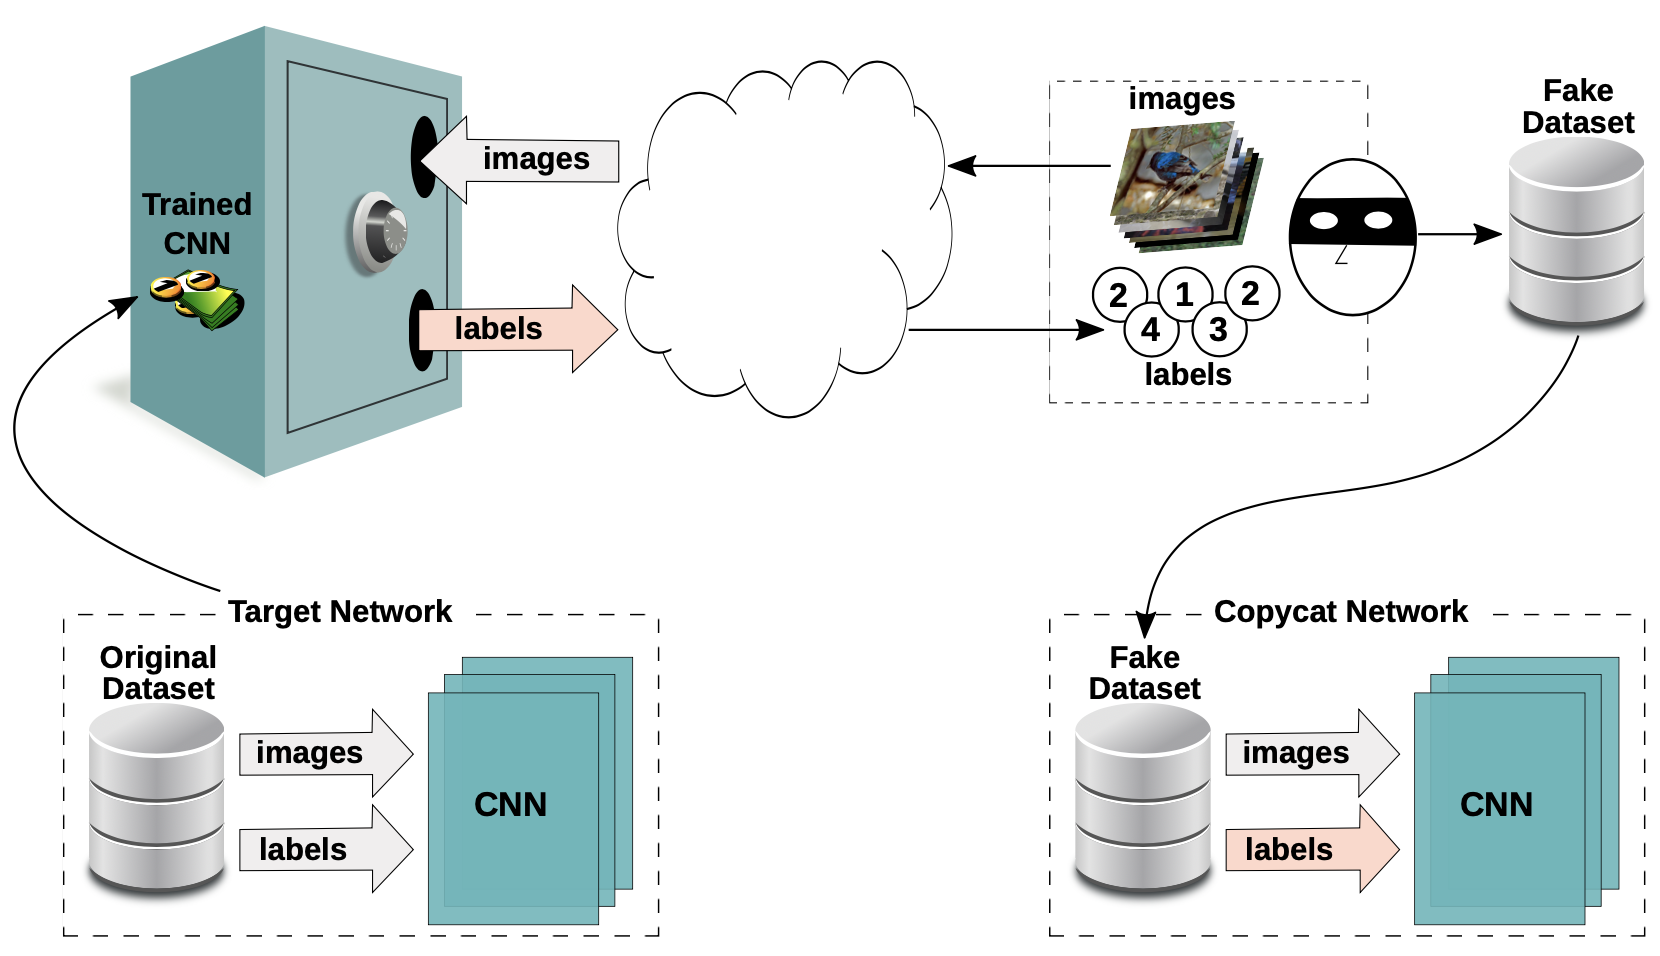
\includegraphics[width=0.75\linewidth]{figures/chapter02/copycatCNN.png}
    \caption{Ataque que realiza CopyCat CNN. \\Fuente: CopyCat CNN \cite{Correia_Silva_2018}}
    \label{fig:copycatcnn}
\end{figure}

En el artículo también demostraron que se podía extraer al menos el 93.7\% del rendimiento de los modelos víctima con datos de dominio no problemáticos y al menos el 98.6\% del rendimiento si se usan datos del dominio del problema. Además, se logró extraer el 97.3\% del modelo de \textit{Microsoft Azure Emotion} usando su API.

% endregion subsubsection Extracción

\subsubsection{Inferencia}
% region subsubsection Inferencia
% \paragraph{Inferencia por Atributos}
% \paragraph{Inferencia por Pertenencia}
% \paragraph{Inversión de modelos}
% \paragraph{Reconstrucción}

En el artículo \cite{10.1145/2810103.2813677} se analizan los ataques de inferencia usando árboles de decisión y un conjunto de datos con información médica de unos individuos, estos ataques permiten extraer información sensible o privada sobre los datos de entrenamiento o sobre las instancias (individuos) a partir de un modelo dé \gls{ML}.

En el artículo se menciona los ataques de inversión de modelo, dicho ataque implica que un atacante abusa del acceso al modelo para extraer información sensible, en concreto habla sobre extraer información genómica sensible de pacientes.

Además, también menciona que se puede extraer los valores de confianza revelados junto con las predicciones, es decir, el nivel de confianza de las predicciones, menciona que se puede usar este dato para inferir información sensible sobre los individuos.

En el artículo \cite{choquettechoo2021labelonly} se mencionan los ataques de inferencia de membresía, estos ataques permiten extraer si una instancia se utilizó para entrenar el modelo. Esto es porque explotan la confianza anormal de los modelos cuando se utilizan instancias del entrenamiento en el modelo entrando. Estos ataques no se pueden usar si el atacante solo obtiene información de la etiqueta y no de la medida de confianza.

En el artículo presentan ataques de membresía usando únicamente etiquetas sin los valores de confianza que estudios anteriores si necesitaban. Esto lo logran evaluando las etiquetas predichas por el modelo en función de determinadas perturbaciones de una instancia.

Ciertas defensas contra estos ataques es la ocultación o alteración del nivel de confianza, en el artículo señalan que los ataques de inferencia de membresía por etiqueta anulan las defensas. Uno de los descubrimientos más relevantes de dicha investigación es que las únicas estrategias de defensas que previenen con éxito todos los ataques son los modelos de entrenamiento con privacidad diferencial y regularización ${L_{2}}$.

% endregion subsubsection Inferencia
